\section{Module de croissance du zooplancton}

\subsection{Description du module}
\par{
Dans les travaux pratiques précédents on a analysé la croissance du phytoplancton en fonction des
nutriments disponibles. Dans les modèles actuels nous sommes moins intéressés par l'approvisionnement
alimentaire du phytoplancton. Nous avons plutôt procédé par enquêter l'interaction du phytoplancton avec
un prédateur naturel de cette espèce, le zooplancton. En conséquence le modèle mathèmatique a été simplifié
de manière à ce qu'on considère maintenant une offre des nutriments infiniment grand pour le
phytoplancton\footnote{En d'autres termes, la croissance du phytoplancton n'est plus limitée par les
nutriments}.
\par{
Pour mieux interpréter les simulations du modèle mathématique nous avons émis l'hypothèse que la mortalité
du phytoplancton est uniquement due au broutage du zooplancton. La mortalité du phytoplancton par d'autres
prédateurs, toxines environnementales, lyse cellulaire etc. n'est pas représentée par le modèle.
Nous supposons donc que l'influence de ces causes de mortalité peut être négligée par rapport à l'influence
de la mortalité de phytoplancton due au broutage du zooplancton.
}
\par{
En résumé, nous obtenons le modèle conceptuel effectué dans la figure~\ref{fig:partie1DiagConcept}
et les équations suivantes:
}

\begin{equation}
  {{d[DA]}\over{dt}} =
  \mu_{DA} [DA] - graz_{MSZ} [MSZ]
  \label{eq:partie1DiffEq1}
\end{equation}
\begin{equation}
  {{d[MSZ]}\over{dt}} =
  \left (
    (1- eges_{MSZ}) graz_{MSZ} Y_{MSZ} - mm_{MSZ}
  \right ) [MSZ]
  \label{eq:partie1DiffEq2}
\end{equation}

\par{
Dans la première partie des travaux pratiques, l'intérêt principal est de comparer l'impacte de la
fonctions de broutage. Pour les analyses, les fonctions de broutage suivantes ont été considérées:
}

\begin{equation}
  \text{Michaelis Menton:~~~}
  graz_{MSZ} = g_{MSZ} \max(T) {{[DA]}\over{kg_{MSZ}+[DA]}}
  \label{eq:partie1GrazMic}
\end{equation}
\begin{equation}
  \text{Michaelis Menton avec seuil:~~~}
  graz_{MSZ} = g_{MSZ} \max(T) {{[DA]-[DA_0]}\over{kg_{MSZ}+([DA]-[DA_0])}}
  \label{eq:partie1GrazMicSeul}
\end{equation}
\begin{equation}
  \text{Holling:~~~}
  graz_{MSZ} = g_{MSZ} \max(T) {{[DA]^2}\over{kg_{MSZ}^2+[DA]^2}}
  \label{eq:partie1GrazHol}
\end{equation}

\begin{figure}[h!]
  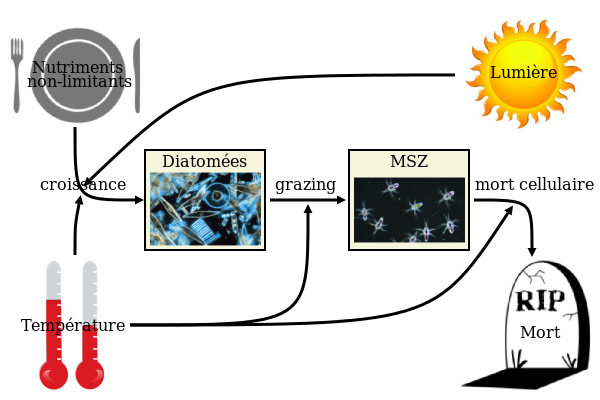
\includegraphics[width=\textwidth]{partie1/diagrammeConceptuel.png}
  \caption{Le modèle conceptuel du système étudié dans le quatrième cours. La croissance du phytoplancton
n'est plus limitée par les nutriments disponibles. Cependant, la croissance est toujours limitée par la
disponibilité de la lumière et de la température. Dans les formules, l'influence de ces deux impacts
environnementals est cachée dans le terme $\mu_{DA}$. Une partie du phytoplancton existant est consommer
par le mésozooplancton (=MSZ). Cette partie est représentée par les fonctions de broutage
différentes fois la concentration du mésozooplancton ($graz_{MSZ}[MSZ]$). Dans le système modèlise
le mésozooplancton n'a pas des prédateurs naturels. Donc, la mort cellulaire naturelle du zooplancton ne peut
plus être négligée (dans les formules c'est le terme $mm_{MSZ}$ qui décrit cette l'influence).
}
  \label{fig:partie1DiagConcept}
\end{figure}

\par{
Pour peut mieux comprendre les équations du modèle, la grille~\ref{tab:partie1signifParam} peut également
être intéressante. Elle donne un aperçu de la signification etc. de chaque terme dans les équations.
}
\par{
Nous voulons encore pointer que $T_{opt}$ et $d_{opt}$ ont les mêmes valeurs pour les diatomées et le
mésozooplancton simulés. On a donc considerer que les deux espèces sont limitées par la tempèrature
de la même façon.
}

\begin{table}[h!]
\begin{center}
\begin{tabular}{ | c | c | c | c | c | }
\hline
Terme & Signification & Type & Valeur & Unité \\
\hline
$[DA]$ & \pbox{4cm}{Concentration du carbon des diatomées} & Variable d'état & $5$ & ${{mmol C}\over{m^{-3}}}$ \\
$[MSZ]$ & \pbox{4cm}{Concentration du carbon du mésozooplancton}  & Variable d'état & $1$ & ${{mmol C}\over{m^{-3}}}$ \\
$\mu_{DA}$ & \pbox{4cm}{Taux de croissance des diatomées} & \pbox{3cm}{Fonction $\mu_{max}max(T)llum$} & \pbox{4cm}{Dépend de la disponibilité de la lumière (en fonction du $[DA]$) et de la tempèrature} & $Jour^{-1}$ \\
$graz_{MSZ}$ & \pbox{4cm}{Fonction de grazing} & Fonction & \pbox{4cm}{Dépend de la tempèrature et de $[DA]$} & $Jour^{-1}$ \\
$eges_{MSZ}$ & \pbox{4cm}{Taux d'egestion du mésozooplancton} & Paramètre & $0.1$ & $-$ \\
$Y_{MSZ}$ & \pbox{4cm}{Efficience de croissance du mésozooplancton} & Paramètre & $0.25$ & $-$ \\
$mm_{MSZ}$ & \pbox{4cm}{Taux de mortalité du mésozooplancton} & Paramètre & $0.05$ & $Jour^{-1}$ \\
$g_{MSZ}$ & \pbox{4cm}{Taux de grazing maximal} & Paramètre & $1.2$ & $Jour^{-1}$ \\
$max(T)$ & \pbox{4cm}{Fonction de la limitation de la tempèrature} & \pbox{3cm}{Fonction\\(bell-shaped)} & \pbox{4cm}{Dépend de $T, T_{opt}$ et $d_{opt}$} & $-$ \\
$kg_{MSZ}$ & \pbox{4cm}{Constante de grazing} & Paramètre & $10$ & ${{mmol C}\over{m^{-3}}}$ \\
$[DA_0]$ & \pbox{4cm}{Concentration minimale avant le mésozooplancton commencent de consummer les diatomées} & Paramètre & $5$ & ${{mmol C}\over{m^{-3}}}$ \\
$\mu_{max}$ & \pbox{4cm}{Taux de croissance maximal des diatomées} & Paramètre & $1.2$ & $Jour^{-1}$ \\
$T_{opt}$ & \pbox{4cm}{Température optimale (pour les diatomées et du mésozooplancton)} & Paramètre & $16.3$ & $^{\circ}C$ \\
$d_{opt}$ & \pbox{4cm}{Delta T (pour les diatomées et du mésozooplancton)} & Paramètre & $13.7$ & $^{\circ}C$ \\
$T$ & \pbox{4cm}{Température simulée} & Paramètre & $10.0$ & $^{\circ}C$ \\
$llum$ & \pbox{4cm}{Limitation par la lumière} & \pbox{3cm}{Fonction\\$1-e^{-\alpha PAR_Z / \mu_{max}}$} & \pbox{4cm}{Dépend de la lumière disponible, ...} & $-$ \\
\end{tabular}
\end{center}
\end{table}
\clearpage
\begin{table}[h!]
\begin{center}
\begin{tabular}{ | c | c | c | c | c | }
$\alpha$ & \pbox{4cm}{L'efficacité des chloroplastes des diatomées} & Paramètre & $0.02$ & ${mol^{-1}*m^2*sec}\over{quanta * jour}$ \\
$PAR_Z$ & \pbox{4cm}{Lumière disponible par mol chlorophylle} & \pbox{3cm}{Fonction\\$PAR_0*e^{-k_e*z}$} & \pbox{4cm}{Dépend de la latitude, les solides en suspension, ...} & ${mol*quanta}\over{m^2*sec}$ \\
$PAR_0$ & \pbox{4cm}{Lumière solaire incidente} & Paramètre & $23.0$ & ${quanta}\over{m^2*sec}$ \\
$k_e$ & \pbox{4cm}{Coefficient d'extinction verticale de la lumière} & \pbox{3cm}{Fonction\\$0.35+0.02{{1}\over{2}}[DA]$} & \pbox{4cm}{Dépend des solides en suspension, ...} & $^{mol}/_m$ \\
$z$ & \pbox{4cm}{Profondeur de l'habitat} & Paramètre & $1.0$ & $m$ \\
\hline
\end{tabular}
\end{center}
  \caption{Signification, type, valeur et unité de chaque terme/paramètre dans les
équations~\ref{eq:partie1DiffEq1},~\ref{eq:partie1DiffEq2},~\ref{eq:partie1GrazMic},~\ref{eq:partie1GrazMicSeul} et~\ref{eq:partie1GrazHol}.}
  \label{tab:partie1signifParam}
\end{table}
\FloatBarrier

\subsection{Analyse mathèmatique}

\par{
La grille~\ref{tab:partie1etatsStat} donne un aperçu des états stationnaires du système
pour les fonctions de broutage diffèrente. Les constantes supplémentaires utilisées
dans la grille sont définies comme suit:
}
\[
m = mm_{MSZ_{MAX_0}} e ^{- \left ( {{t-t_{opt}}\over{d_{opt}}} \right )}
\]
\[
k = kg_{MSZ}
\]
\[
c = \left ( 1 - eges_{MSZ} \right ) y_{MSZ}
g_{MSZ_{MAX_0}} e ^{- \left ( {{t-t_{opt}}\over{d_{opt}}} \right )}
\]
\[
f = g_{MSZ_{MAX_0}} e ^{- \left ( {{t-t_{opt}}\over{d_{opt}}} \right )}
\]

\begin{table}[h!]
\begin{center}
\begin{tabular}{ | c | c c | }
\hline
fct. de broutage & $[DA]$ & $[MSZ]$ \\
\hline
MIC, MIC\_Seul, HOL & 0 & 0 \\
MIC & $k * {{m}\over{c-m}}$ & ${{\mu_{DA} k \left ( 1 + {{m}\over{c-m}} \right )}\over{f}}$ \\
MIC\_Seuil & ${{m/c*k-m/c[DA_0]+[DA_0]}\over{1-m/c}}$ & ${\mu_{DA} * [DA] * (k + [DA] - [DA_0])}\over{f *([DA] - [DA_0])}$ \\
HOL & $k*\sqrt{{{m}\over{c-m}}}$ & ${{\mu_{DA}k \left ( 1 + {m}\over{c-m} \right )}\over{f \sqrt{{m}\over{c-m}}}}$ \\
\hline
\end{tabular}
\end{center}
  \caption{Les états stationnaires du système pour les fonctions de broutage diffèrente. Les
constantes supplémentaires utilisées ont était définies dans le texte précédent. Les formules sont en accord
avec les simulations informatiques décrites ci-dessous (cmp grille~\ref{tab:partie1appPropFctGrazing} et
figure~\ref{fig:partie1RefSimulations}).
}
  \label{tab:partie1etatsStat}
\end{table}
\FloatBarrier

\par{
Pas tous les états stationnaires listent dans la table~\ref{tab:partie1etatsStat} sont stables. Pour
étudier la stabilité des états stationnaires différents on doit établir la matrice jacobienne.
Malheureusement il nous a manque un peu du temps pour etudier la stabilité en détail.
}

\subsection{Comparision des fonction de grazing diffèrente}

\par{
Dans une première étappe l'aissez nous discouter l'impact de la fonction de grazing. La courbe de les
trois fonction diffèrente a était tracée dans la figure~\ref{fig:partie1grazingFcts}.
On peut observer les propriétés suivantes:
}
\begin{itemize}
  \item Toutes les courbes sont en augmentation monotone et s'approchent à un taux croissance de valeur
$g_{MSZ} max(T)$. La dérivée seconde des équations~\ref{eq:partie1GrazMic} et~\ref{eq:partie1GrazMicSeul}
est strictement négatif. En conséquence les courbes sont courbées vers la gauche. Au contraire, la
dérivée seconde de l'équation~\ref{eq:partie1GrazHol} est positive entre $[0, kg_{MSZ}]$
et négatif dans la région $[kg_{MSZ}, \infty[$. Alors pour tous les valeurs dans la zone $[-kg_{MSZ},kg_{MSZ}]$
la courbe est courbée vers la gauche. En dehors de cette région la courbe est courbée vers la droite.
  \item Quand on est à des concentrations des diatomées faibles, l'équation~\ref{eq:partie1GrazMic}
donne le taux croissance le plus élevé. Lorsque la concentration des diatomées dépasse $kg_{MSZ}$,
l'équation~\ref{eq:partie1GrazHol} donne le taux croissance le plus élevé.
  \item La courbe de l'équation~\ref{eq:partie1GrazMicSeul} est déplace par rapport de la
courbe de l'équation~\ref{eq:partie1GrazMic} sur l'axe des abscisses par $[DA_0]$. Par conséquent,
les courbes de l'équation~\ref{eq:partie1GrazMic} et de l'équation~\ref{eq:partie1GrazMicSeul}
se croisent seulement à l'infini.
  \item Les courbes de les équations~\ref{eq:partie1GrazMicSeul} et~\ref{eq:partie1GrazHol}
ne se croissent pas dans la région $[0, \infty[$ quand $[DA_0]$ et supérieur à $0.25$.
(Point(s) d'intersection: $x = {^1/_2} \left ( 1 \pm \sqrt{1 - 4 [DA_0]}\right )$).
\end{itemize}

\begin{figure}[h!]
  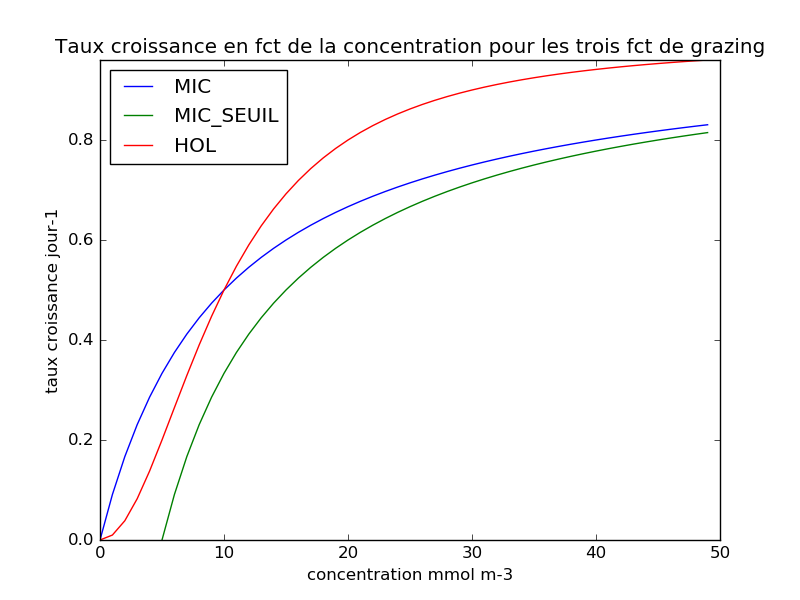
\includegraphics[width=\textwidth]{partie1/grazingFct.png}
  \caption{
La courbe de les trois fonctions~\ref{eq:partie1GrazMic} (MIC),~\ref{eq:partie1GrazMicSeul} (MIC\_SEUIL)
et~\ref{eq:partie1GrazHol} (HOL) en fonction de la concentration $[DA]$.
}
  \label{fig:partie1grazingFcts}
\end{figure}

\par{
En utilisation ces propriétés, nous pouvons maintenant discouter certains simulations (voir
figure~\ref{fig:partie1RefSimulations}) pour étudier mieux l'impact de la fonction de grazing.
Le tableau~\ref{tab:partie1appPropFctGrazing} donne une vue synoptique sur les maximas et l'état
stationnaire du modèle pour les fonction de grazing étudiées.
}
\begin{table}[h!]
\begin{center}
\begin{tabular}{ | c | c c | c c | c c |}
\hline
Fonction & \multicolumn{2}{c|}{Maximum $[DA]$} & \multicolumn{2}{c|}{Maximum $[MSZ]$} &
\multicolumn{2}{c|}{État stat.} \\
de grazing & Temps & Conc. & Temps & Conc. & $[DA]$ & $[MSZ]$ \\
\hline
MIC (voir eq.~\ref{eq:partie1GrazMic}) & $21.84$ & $87.474$ & $30.36$ & $39.992$ & $0.0$ & $0.0$ \\
MIC\_SEUIL (voir eq.~\ref{eq:partie1GrazMicSeul}) & $22.86$ & $112.107$ & $32.04$ & $45.979$ & $7.273$ & $10.478$ \\
HOL (voir eq.~\ref{eq:partie1GrazHol}) & $18.42$ & $60.979$ & $25.44$ & $29.276$ & $4.767$ & $7.016$ \\
\hline
\end{tabular}
\end{center}
  \caption{Les simulations (cmp figure~\ref{fig:partie1RefSimulations}) montrent des maximas et
des état stationnaire différents. Ce tableau donne une vue synoptique sur les maximas
(temps et concentration) et l'état stationnaire du modèle pour les fonctions de grazing différente
(cmp fonctions~\ref{eq:partie1GrazMic},~\ref{eq:partie1GrazMicSeul} et~\ref{eq:partie1GrazHol}).}
  \label{tab:partie1appPropFctGrazing}
\end{table}

\par{
\todo
}

\begin{figure}[h]
  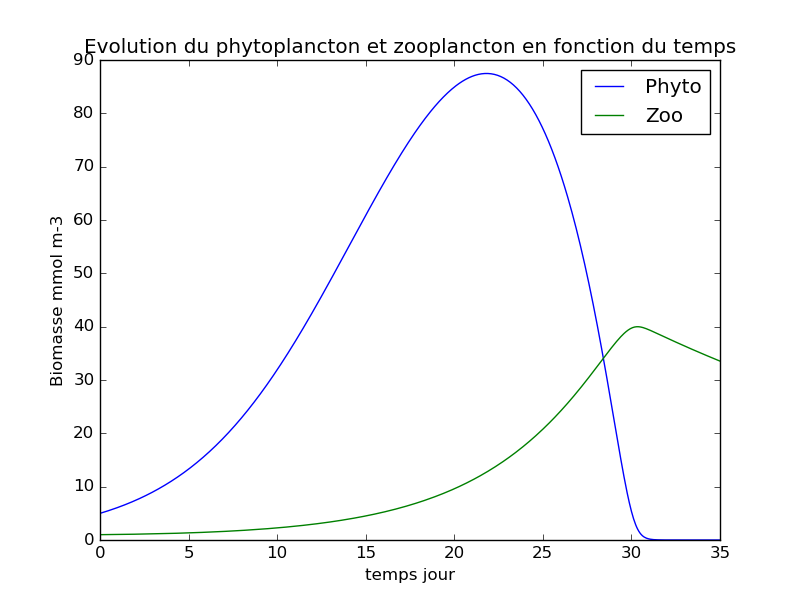
\includegraphics[width=0.5\textwidth]{partie1/refMic35.png}\hfill
  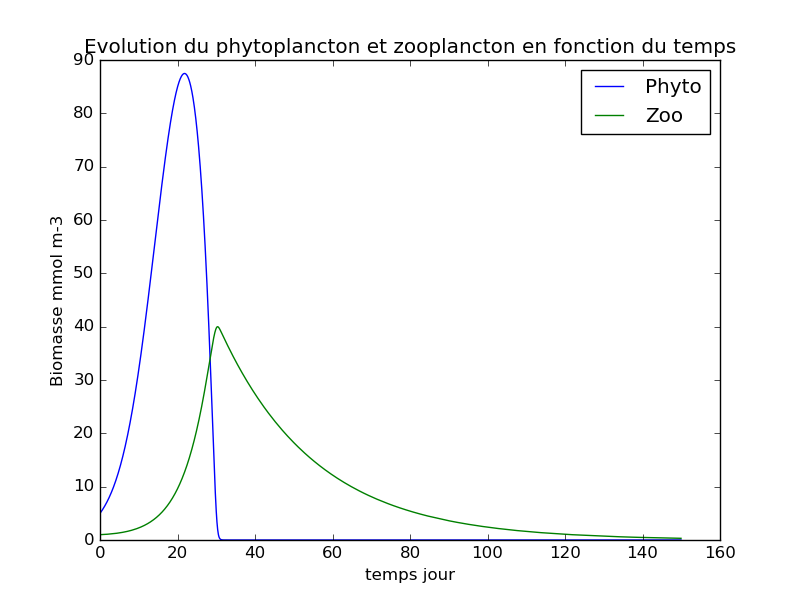
\includegraphics[width=0.5\textwidth]{partie1/refMic150.png}\\
  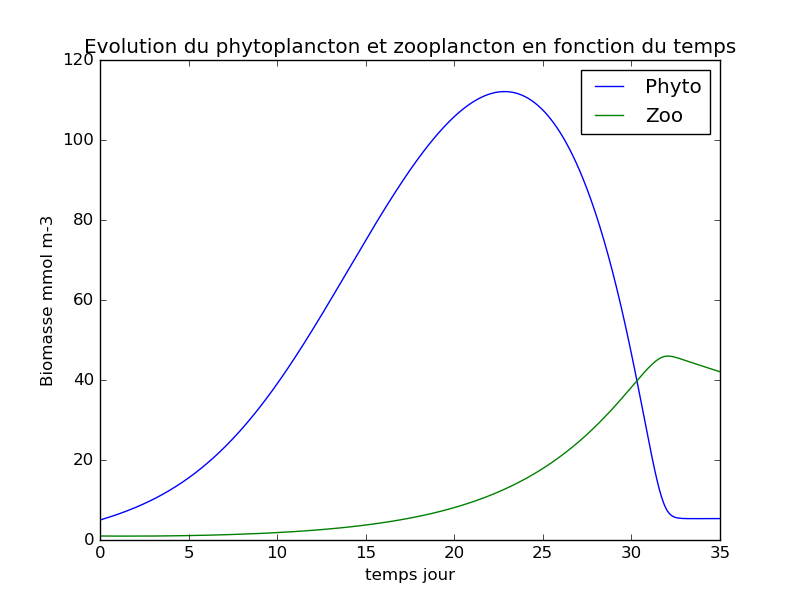
\includegraphics[width=0.5\textwidth]{partie1/refMicSeul35.png}\hfill
  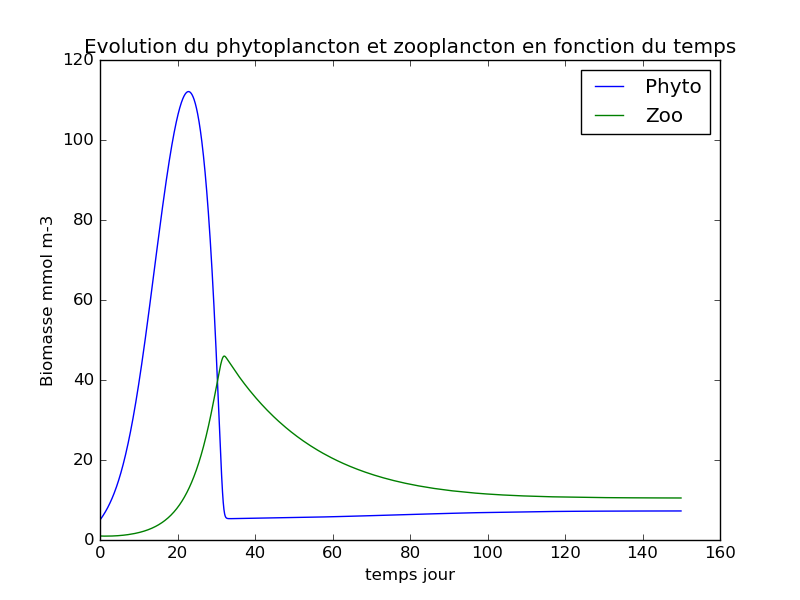
\includegraphics[width=0.5\textwidth]{partie1/refMicSeul150.png}\\
  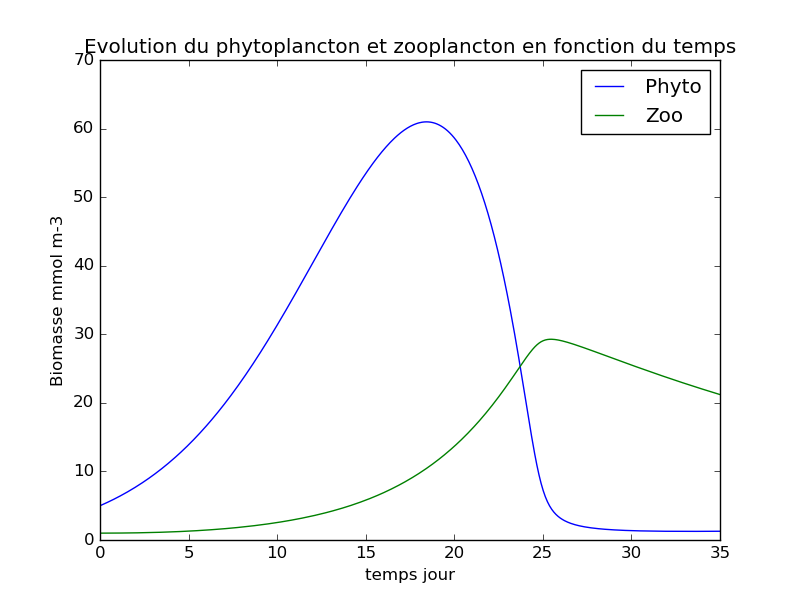
\includegraphics[width=0.5\textwidth]{partie1/refHol35.png}\hfill
  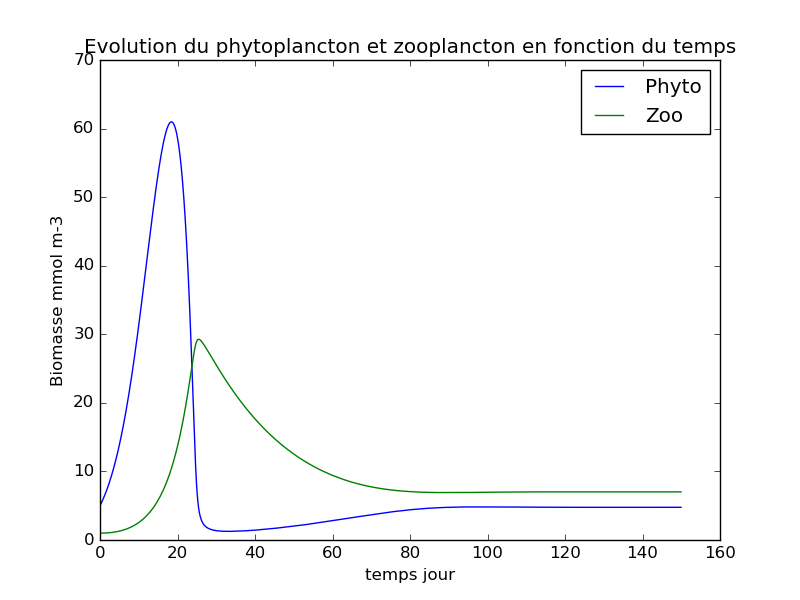
\includegraphics[width=0.5\textwidth]{partie1/refHol150.png}
  \caption{Les simulations de références pour les fonctions diffèrente de grazing (
fonction de Michaelis-Menton (eq.~\ref{eq:partie1GrazMic}, première ligne),
Michaelis-Menton avec seuil (eq.~\ref{eq:partie1GrazMicSeul}, deuxième ligne) et fonction de
Holling (eq.~\ref{eq:partie1GrazHol}, ligne terminale)) pour des temps final diffèrente.
Avec un temps final de 35 jours la colonne de gauche montre une sous-partie des graphiques
de la colonne de droite. La colonne de droite montre le cours de simulation jusqu'à un temps
final de 150 jours.}
  \label{fig:partie1RefSimulations}
\end{figure}

\clearpage
\subsection{Changements des paramètres}




\subsection{Conclusion}
